%!TEX root = ../thesis.tex
%*******************************************************************************
%*********************************** Introduction *****************************
%*******************************************************************************

\chapter{Introduction}
\label{chap:introduction}
\ifpdf
    \graphicspath{{Chapters/Introduction/Figs/}{Chapters/Introduction/Figs/}{Chapters/Introduction/Figs/}}
\else
    \graphicspath{{Chapters/Introduction/Figs/}{Chapters/Introduction/Figs/}}
\fi
This chapter aims to provide an introduction to the main topics and objectives of this master thesis. 
First, we present the motivation behind our work (see section \ref{introduction:section:motivation}), highlighting the importance of \ac{ui} design in software development and the challenges that arise in this context.
Then, we define three problem statements (see section \ref{introduction:section:problems}) related to \ac{ui} prototyping and \ac{ui} experimentation. 
Next, we explain our research approach (see section \ref{introduction:section:research}) methodology and define the \ac{rq} that guides our investigation. 
After that, we describe our solution approach (see section \ref{introduction:section:solution}), consisting of a systematic study using the LEAN development cycle. 
Finally, we outline the structure of the thesis (see section \ref{introduction:section:structure}), providing an overview of the main chapters and their contents.

%********************************** % Motivation  **************************************
\section{Motivation} % Section - 1.1 
\label{introduction:section:motivation}

Over the last decade, software development had a tremendous impact with increasing customer demand and requirements \cite{article:swdemand:ahmed}, further increasing product complexity and ambiguity, significantly impacting software development.
As a result, it is increasingly more work for developers to assess user requirements and opinions, leading to biases towards certain requirements and overlooking user needs.
Therefore, to meet these requirements, developers have devised various techniques to obtain early user feedback from potential customers \cite{misc:expperiments:split}. 
At the same time, traditional \ac{ui} prototyping tools rely on manual and time-consuming processes, making it difficult to obtain early user feedback in the product development phase \cite{paper:prototyping:luqi}.
Therefore, the developers have devised different techniques to meet this requirement criteria, including new approaches to \ac{ui} prototyping.
\begin{figure}[ht]
    \centering
    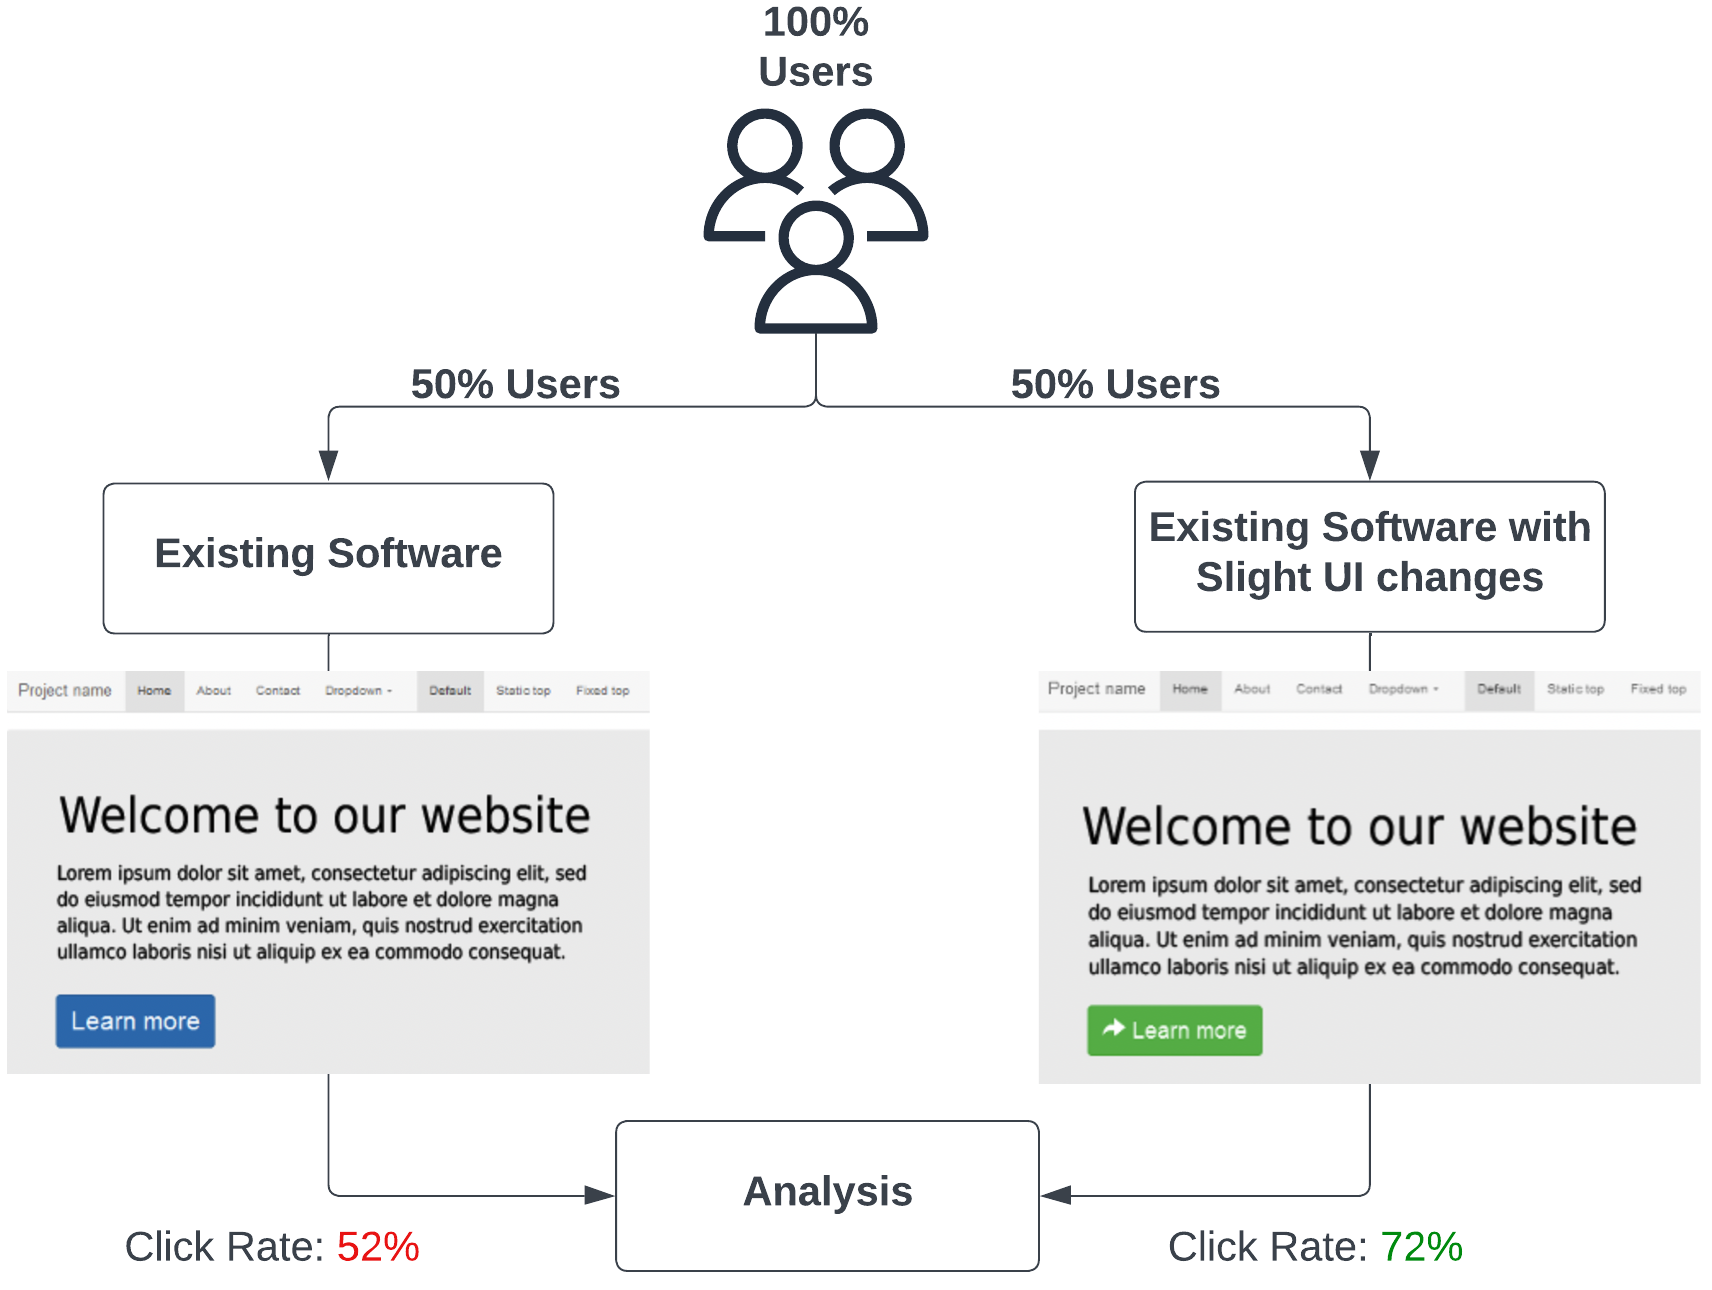
\includegraphics[scale=0.17]{splittesting.png}
    \caption[Split Testing]{UI Experimentation Overview \cite{misc:expperiments:split}}
    \label{intro:fig:splittesting}
\end{figure}

Early user feedback from potential customers in the industry is crucial for creating successful software products, given the growing market uncertainties and consumers' desire for integrated solutions to their issues \cite{misc:businessmodels:teece}.
Therefore, giving users a ``partially functioning'' system is the most excellent method to determine their requirements and suggestions \cite{journal:prototyping:davis}.
This ensures that the developers with high uncertainties in the early product development phase can improve the product by testing the underlying assumptions \cite{misc:lean:steve}.
Developers can use this feedback to validate the most critical assumptions about the software product. 
This validation can decide whether to add, remove or update a feature \cite{article:experiments:lindgren}. 

This process of determining the best fit for the product through user feedback is called \ac{ui} experimentation or split testing.
In split testing (see figure \ref{intro:fig:splittesting}), the \ac{ux} designers design different UI variants (e.g., buttons with different colors), and the developer integrates these variants and assigns them to a distinct group of users. 
As per some evaluation criteria (e.g., more clicks on the button), the variant with better results is deployed for the entire population or all the users.
Software products have shown the benefits of conducting experiments in many use cases with incremental product improvement \cite{article:controlled:experiements}.
There has been an increase in interest in the types of experimentation that can take place in product development. 
So, an experiment can be valuable when it improves the software products.
However, many \ac{ui} experimentation techniques \cite{article:controlled:experiements, article:experiments:lindgren} usually involve only quantitative analysis, which has several disadvantages. 
One of the main drawbacks of using only quantitative analysis is that it fails to provide insights into the underlying reasons for user behavior \cite{article:qqa:young}. 
For example, a high bounce rate on a particular page could be due to several factors, such as poor navigation, slow loading times, or unappealing design \cite{article:right:model}. 
Without qualitative feedback, it can be challenging to pinpoint the exact cause of the problem and make the necessary improvements \cite{article:qq:helena}.
Based on these identified challenges, we define problem statements in the next section.


% In conclusion, we propose an iterative UI prototyping approach that allows developers to incorporate user feedback throughout the development process, resulting in a product that meets the needs of the end users. 
% We also suggest incorporating different UI variants in the UI prototyping approach to test which design performs best. 
% At the same time, combine qualitative and quantitative analysis from user feedback in UI experimentation for a more comprehensive understanding of user needs. 
% By implementing these approaches, developers can create more user-focused software products, leading to higher user satisfaction and overall project success.
% Software development has seen an increasing demand for product complexity and ambiguity in the past decade, which has significantly impacted the development process. To meet these requirements, developers have come up with various techniques to obtain early user feedback from potential customers. Early feedback is crucial in creating successful software products due to market uncertainties and customers' desires for integrated solutions to their issues. However, determining user requirements becomes increasingly challenging with the growing complexity of products, making it more difficult for developers to assess user opinions.
% To reduce the risks associated with biased assumptions, developers need to detect user needs and requirements early. One of the most excellent methods to determine these needs and suggestions is by providing users with a partially functioning system. This process allows developers to test underlying assumptions and validate critical assumptions about the software product, deciding whether to add, remove, or update a feature. This process of determining the best fit for the product through user feedback is called experimentation.
% Experimentation has shown its benefits in many use cases, particularly in software product development. In experimentation, designers create different UI variants (e.g., buttons with different colors), and developers integrate these variants and assign them to a distinct group of users. The variant with better results, as per some evaluation criteria (e.g., more clicks on the button), is deployed for the entire set of users. However, creating different UI variants can be time-consuming and require a lot of manual effort, which can slow down the development process.
% To address this issue, a provision in our approach is required to create different UI variants iteratively. In addition, combining qualitative and quantitative analysis in our approach can help make informed decisions and ensure successful experimentation in software development. Our thesis aims to address these three problems in software development, making experimentation more efficient and effective in determining the best fit for a software product.
\clearpage
%********************************** % Problem Statement  *************************************
\section{Problem Statement} % Section - 1.2
\label{introduction:section:problems}
The motivation section shows some gaps in software development between the developers and the designers.
This section aims to highlight the three problems that arise during software development, their corresponding problem statements and a brief solution.

\paragraph{Problem 1:} 
Developing software products that meet customers' needs is crucial for software companies as it is challenging to determine user requirements \cite{article:experiments:lindgren}. 
\ac{ux} designers face a significant problem as they must design software products catering to users' expectations and preferences. 
However, it is difficult to know whether the designed product will meet users' needs without a reliable way to test user responses. 
This challenge is worsened by user requirements and preferences constantly changing, requiring designers to iterate on their designs. 
Therefore, finding a solution to test designs and gather user feedback to build software products that meet users' needs is necessary.

% Product designers create many UI prototypes, and the developers implement them.
% To determine the best variant, the developers create experiments with the users \cite{article:experiments:lindgren}. 
% This concrete implementation of designs uses a lot of resources and time for the developers.
% Therefore, the product designers need to be integrated into the development process so that they would be able to create experiments independently of the developers.

% \paragraph{Problem 2:} When the product designers develop the prototypes, testing them with many users is difficult as the product is still not developed.
% Therefore, it is not easy to conclude a ``winner'' variant with a small amount of data as it is statistically difficult to prove one of the variants outperforms the others \cite{article:usability:smalldata}.
% Therefore, it is necessary to develop an idea that the designers can use to determine the best prototype or variant with a small group of users.

\paragraph{Problem 2:} Most often, the software application collects data from the experiments. 
Some data is used in qualitative analysis, while others are in quantitative analysis.
Many companies fail to reap the benefits of using both qualitative and quantitative analysis.
Similarly, not all the data is used in the analysis phase reducing the software applications to improve based on customer feedback \cite{article:datadrive:brian}.
Therefore, finding a solution that combines qualitative and quantitative data analysis is necessary.

\paragraph{Problem 3:} 
The traditional iterative development approach is based on designing, prototyping, and testing multiple software product versions before arriving at a final version that meets the users' needs \cite{article:experiments:lindgren}.
However, this approach can be time-consuming and inefficient in \ac{ui} prototyping and experimentation as this approach can result in biased decision-making, where developers may ignore valuable feedback from users, resulting in suboptimal results.
Therefore, finding a solution for a more efficient and effective approach to \ac{ui} prototyping and experimentation that overcomes these challenges and ensures optimal design choices is necesary.

\clearpage
%********************************** % Research Approach  *************************************
\section{Research Approach}  % Section - 1.3 
\label{introduction:section:research}
The problems identified in the previous section highlight the need for a research approach that can help address them effectively.
Therefore, in this section, we define \ac{rq}s and highlight our research approach. 
We also define the meanings of \ac{dr}, \ac{dp} and \ac{df} which would be used in further sections.
Our research approach aims to provide a systematic way of developing software products that meet customer needs while minimizing the risk of developing features that may not be useful to end users.

\paragraph{\ac{rq}1:} \textit{What are the most effective techniques and methods for incorporating qualitative and quantitative user feedback into the design process of UI prototypes to improve \ac{ux}?}
\paragraph{\ac{rq}2:} \textit{How to develop a software tool suitable for \ac{ux} designers to conduct experiments on UI prototypes iteratively?}

\begin{figure}[ht]
    \centering
    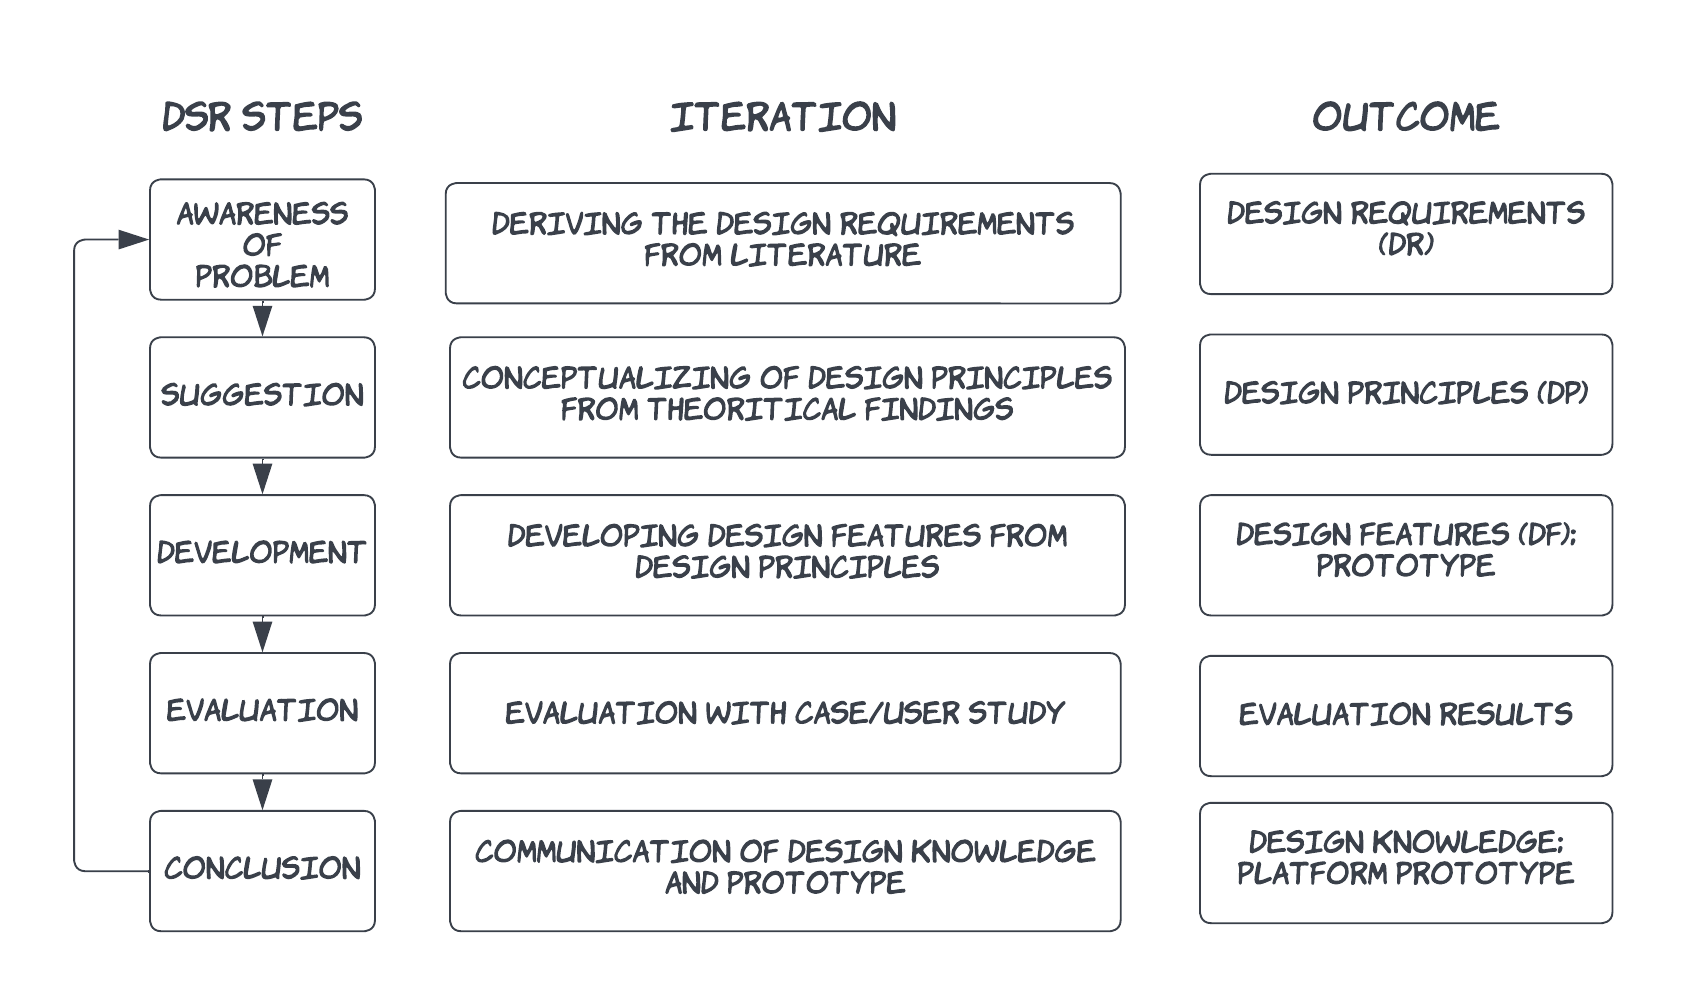
\includegraphics[scale=0.2]{DSRcycle.png}
    \caption[Design Science Research Cycle]{Design Science Research Cycle \cite{paper:designprinciple:vk}}
    \label{intro:fig:dps}
\end{figure}

\ac{dsr} aims to provide prescriptive knowledge about the design of artifacts, such as software techniques, models, or concepts \cite{paper:designprinciple:vk}.
It follows a rigorous problem identification, solution design, implementation, and evaluation process, aiming to produce useful and effective artifacts that address real-world problems \cite{paper:designprinciple:gregor}. 
The approach combines rigorous scientific methods and practical considerations to ensure that the artifacts developed are theoretically sound and useful in practice.
It is an iterative approach involving a problem-solving cycle of developing a solution, evaluating it, and refining it based on feedback. 
In our research, we will conduct the \textit{first} iteration of \ac{dsr} to develop and evaluate a solution that addresses the identified problems and answer the \ac{rq}s.

The DSR approach consists of five steps (see figure \ref{intro:fig:dps}), starting with problem awareness, where we define the problem and gain an understanding of it through studying relevant literature and tools. 
The outcome of this step is the identification of \ac{dr}s. 
In the second step, we concretize the \ac{dr}s to develop \ac{dp}s that serve as guidelines for designing the artifact. 
In the third step, we create \ac{df}s that should be available in the artifact and build the tool.
In the fourth step, we evaluate the tool through a user study to gather feedback and results. 
Finally, in the fifth step, we improve our tool and re-iterate the \ac{dp}s based on the feedback received. 
Through this iterative approach, we aim to develop an effective and user-friendly \ac{ui} prototyping tool that addresses the problems identified in software development.

% As a result, this design and application may provide design-focused information that adds to the DSR knowledge corpus \cite{misc:dsr:henver}.
% Every element within a DSR project is built upon and systematically analyzed to add to the overall DSR knowledge corpus.
% Therefore through the use of \ac{dsr}, a group of issues is resolved by concentrating on a single issue and abstracting the consequences of the resolution.

\paragraph{Design Requirements:}
In \ac{dsr}, abstracted \ac{dr} refer to the general, high-level requirements that a design must meet to succeed \cite{misc:dsr:webster}. 
These requirements are typically derived from the RQ identified as relevant to the problem.
Abstracted \ac{dr}s provide a broad framework for the design process and help to ensure that the design solution addresses the key issues and challenges identified in the research problem. 
They can also help guide the evaluation of the design solution and ensure that the solution is grounded in the \ac{dp}s identified as necessary.

\paragraph{Design Principles:}
In \ac{dsr}, \ac{dp}s refer to specific, detailed guidelines that a design must follow to be successful \cite{misc:dsr:webster}. 
These principles are derived from the abstract \ac{dr}s identified as relevant to the research problem and provide more specific guidance on how the design should be implemented.
\ac{dp}s can also be defined as the codification of our knowledge during the design study while identifying the DRs. 
Concrete DPs are essential in \ac{dsr} as they help ensure that the design solution meets the needs and goals of the research problem and is grounded in the \ac{dp}s we identified as necessary.

\paragraph{Design Features:}
In \ac{dsr}, \ac{df}s refer to the characteristics of the artifacts or solutions created through the process \cite{misc:dsr:webster}. 
These \ac{df}s provide a means of evaluating the solution's effectiveness and can serve as guidelines for others who may want to adopt or modify the solution.
\ac{df}s typically include both functional and non-functional aspects of the solution. 
Functional features relate to the specific capabilities and functionalities that the solution provides whereas, non-functional features relate to characteristics such as usability, scalability, etc. 
By explicitly specifying these \ac{df}s, \ac{dsr} researchers can ensure that their solutions are aligned with the stakeholders' needs and meet the necessary standards of quality and effectiveness.

\clearpage
\section{Solution Overview}
\label{introduction:section:solution}
After identifying the research approach in the previous section, we now present the solution overview of our approach using the LEAN development cycle.
The designers should be able to create UI prototypes and experiments on their own with a set of users.
Since we do not have a large set of users for testing the prototypes, we use supervised task-based usability testing \cite{article:dataanalysis:supervisedtest}.
The fundamental principle of task-based usability testing is to have the users attempt to use the prototypes to do certain activities or tasks (e.g., Locate a comedy movie) and get feedback (e.g., the time required for the task to be completed by the user).
We propose to use a no-code approach to achieve this.
This approach helps to have a \ac{ui} for the designers to understand, develop, and create experiments and tasks with the software prototypes \cite{paper:lowcode:khorram}.
So, the designers would be able to create the \ac{ui} prototypes and their variants, assign them to the users in an experiment, get feedback from the users and decide on the best prototype without writing any code.
At the same time, the no-code has become more accessible for model-driven development \cite{article:lowcode:modeldriven}.
Therefore, we plan to create models for the \ac{ui} prototypes and have the feasibility for creating experiments and tasks. 
Because of using the models, it is easier to store the prototypes in the database and conduct experiments with the users. 
\begin{figure}[ht]
    \centering
    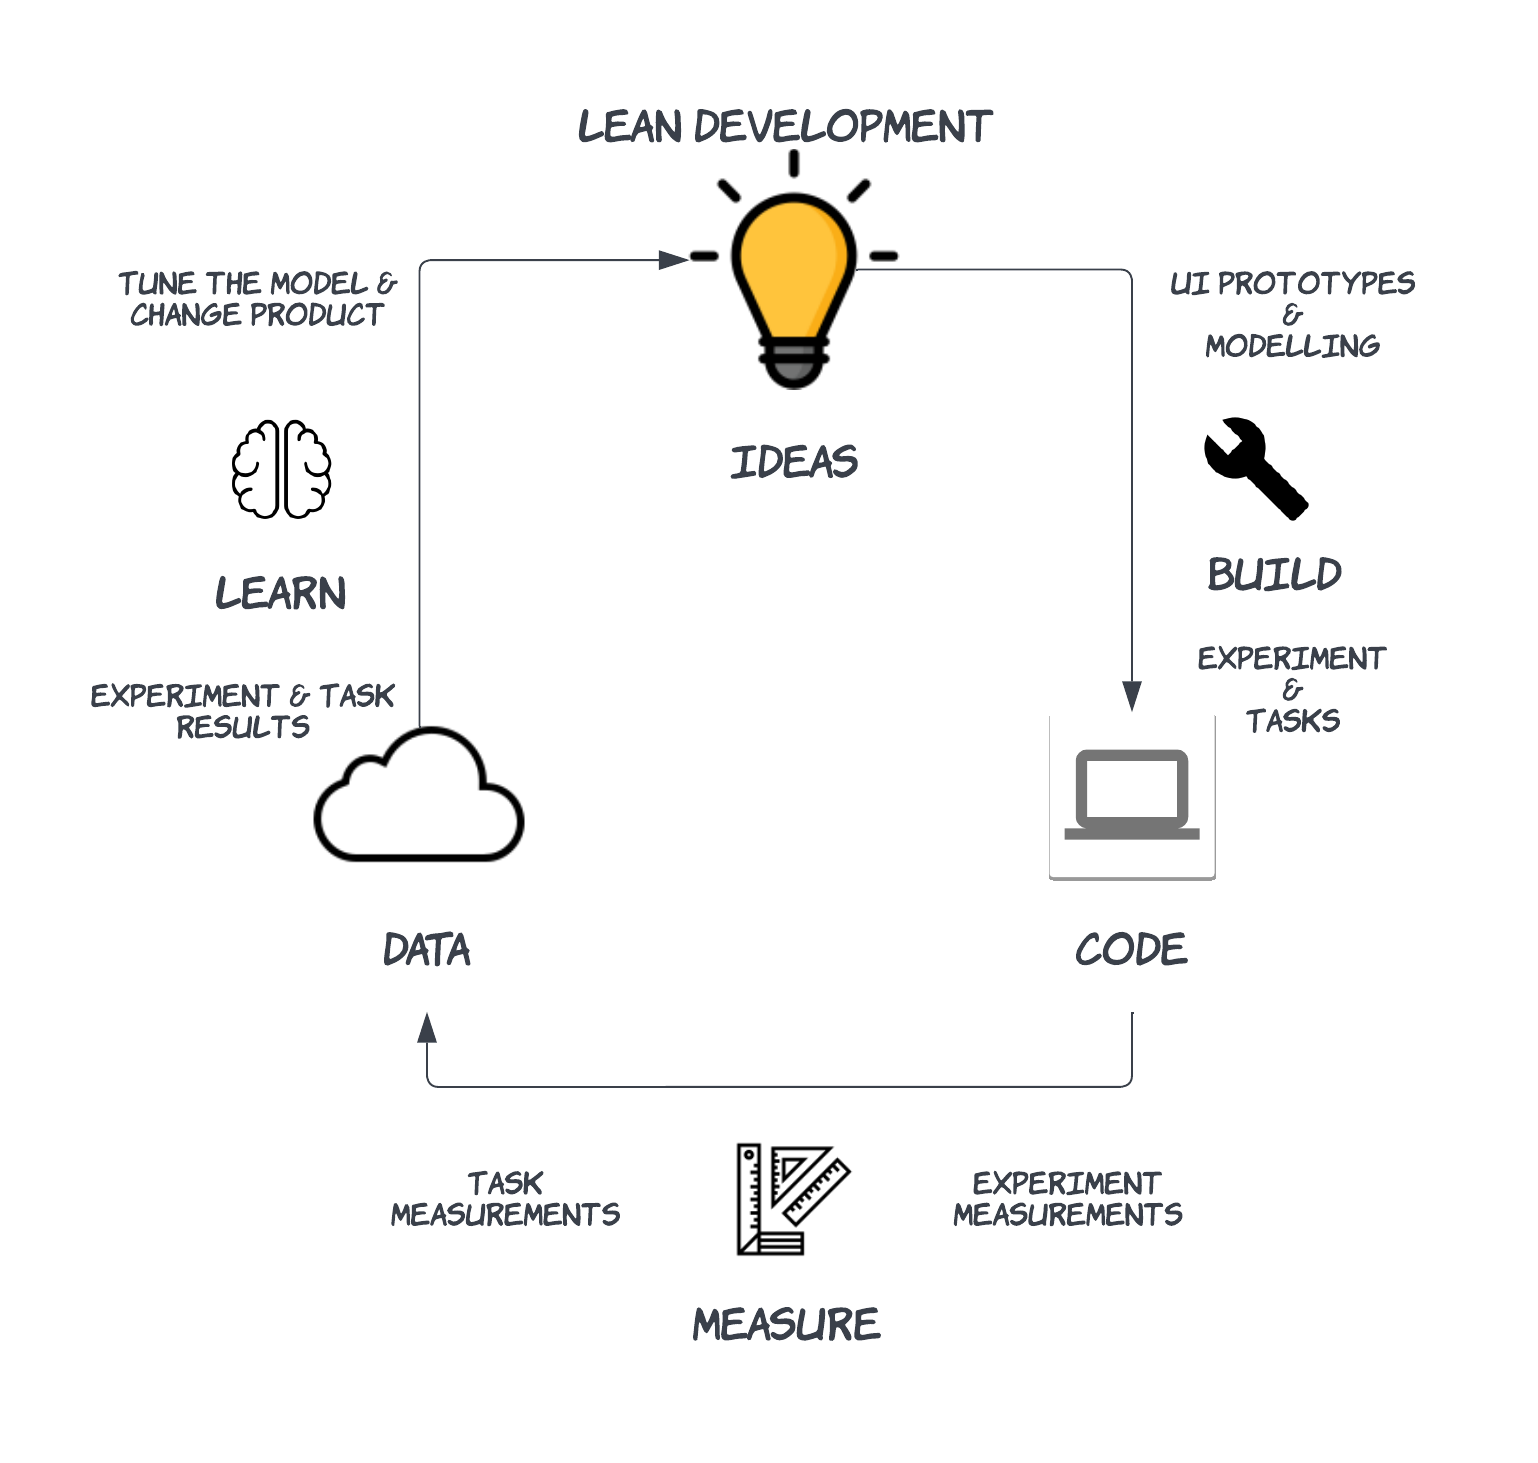
\includegraphics[scale=0.18]{LEAN.png}
    \caption{LEAN Development Technique}
    \label{intro:fig:lean}
\end{figure}

In our solution, we adopt the LEAN development technique (see figure \ref{intro:fig:lean}) for development as it is used to develop user-friendly products \cite{article:lean:hart}.
% Using LEAN, the company creates a \ac{mvp} throughout development, tests it with potential customers, and leverages their input to make incremental changes.
While this technique can be used for every product, there are also approaches specific to software products.
LEAN development technique can be divided into a Build, Measure, and Learn cycle. \\
In the \textit{(1) building} phase, we develop the models for our approach and built a \ac{ui} prototyping tool. 
We then add provisions to create \ac{ui} experiments, user tasks and custom questionnaires to collect user feedback. 
Additionally, we include a provision to assign user participants to the UI variant in an experiment. \\
In the \textit{(2) measurement} phase, after the completion of the experiment, we collect both the user feedback and the qualitative questionnaire answers.
Therefore, the feedback will be both qualitative and quantitative.\\
In the \textit{(3) learning} phase, we analyze the experiment results and determine the better variant based on the feedback collected. 
Based on the findings, we will refine our model and develop the new UI prototypes. 
Our approach using the LEAN development cycle allows us to conduct iterative UI experimentation, leading to improved UI designs that better meet user needs. \\
As per figure \ref{intro:fig:lean}, we complete one cycle of iteration and start a new one with the updated prototype.

\clearpage

\section{Thesis Structure}
\label{introduction:section:structure}
The structure of our thesis is designed to provide a comprehensive overview of our research and solution approach.
The \textit{\hyperref[chap:introduction]{(1) Introduction}} chapter includes a detailed analysis of the problem statement, motivation, research question, and our research and solution approach.

\begin{figure}[htbp!]
    \centering
    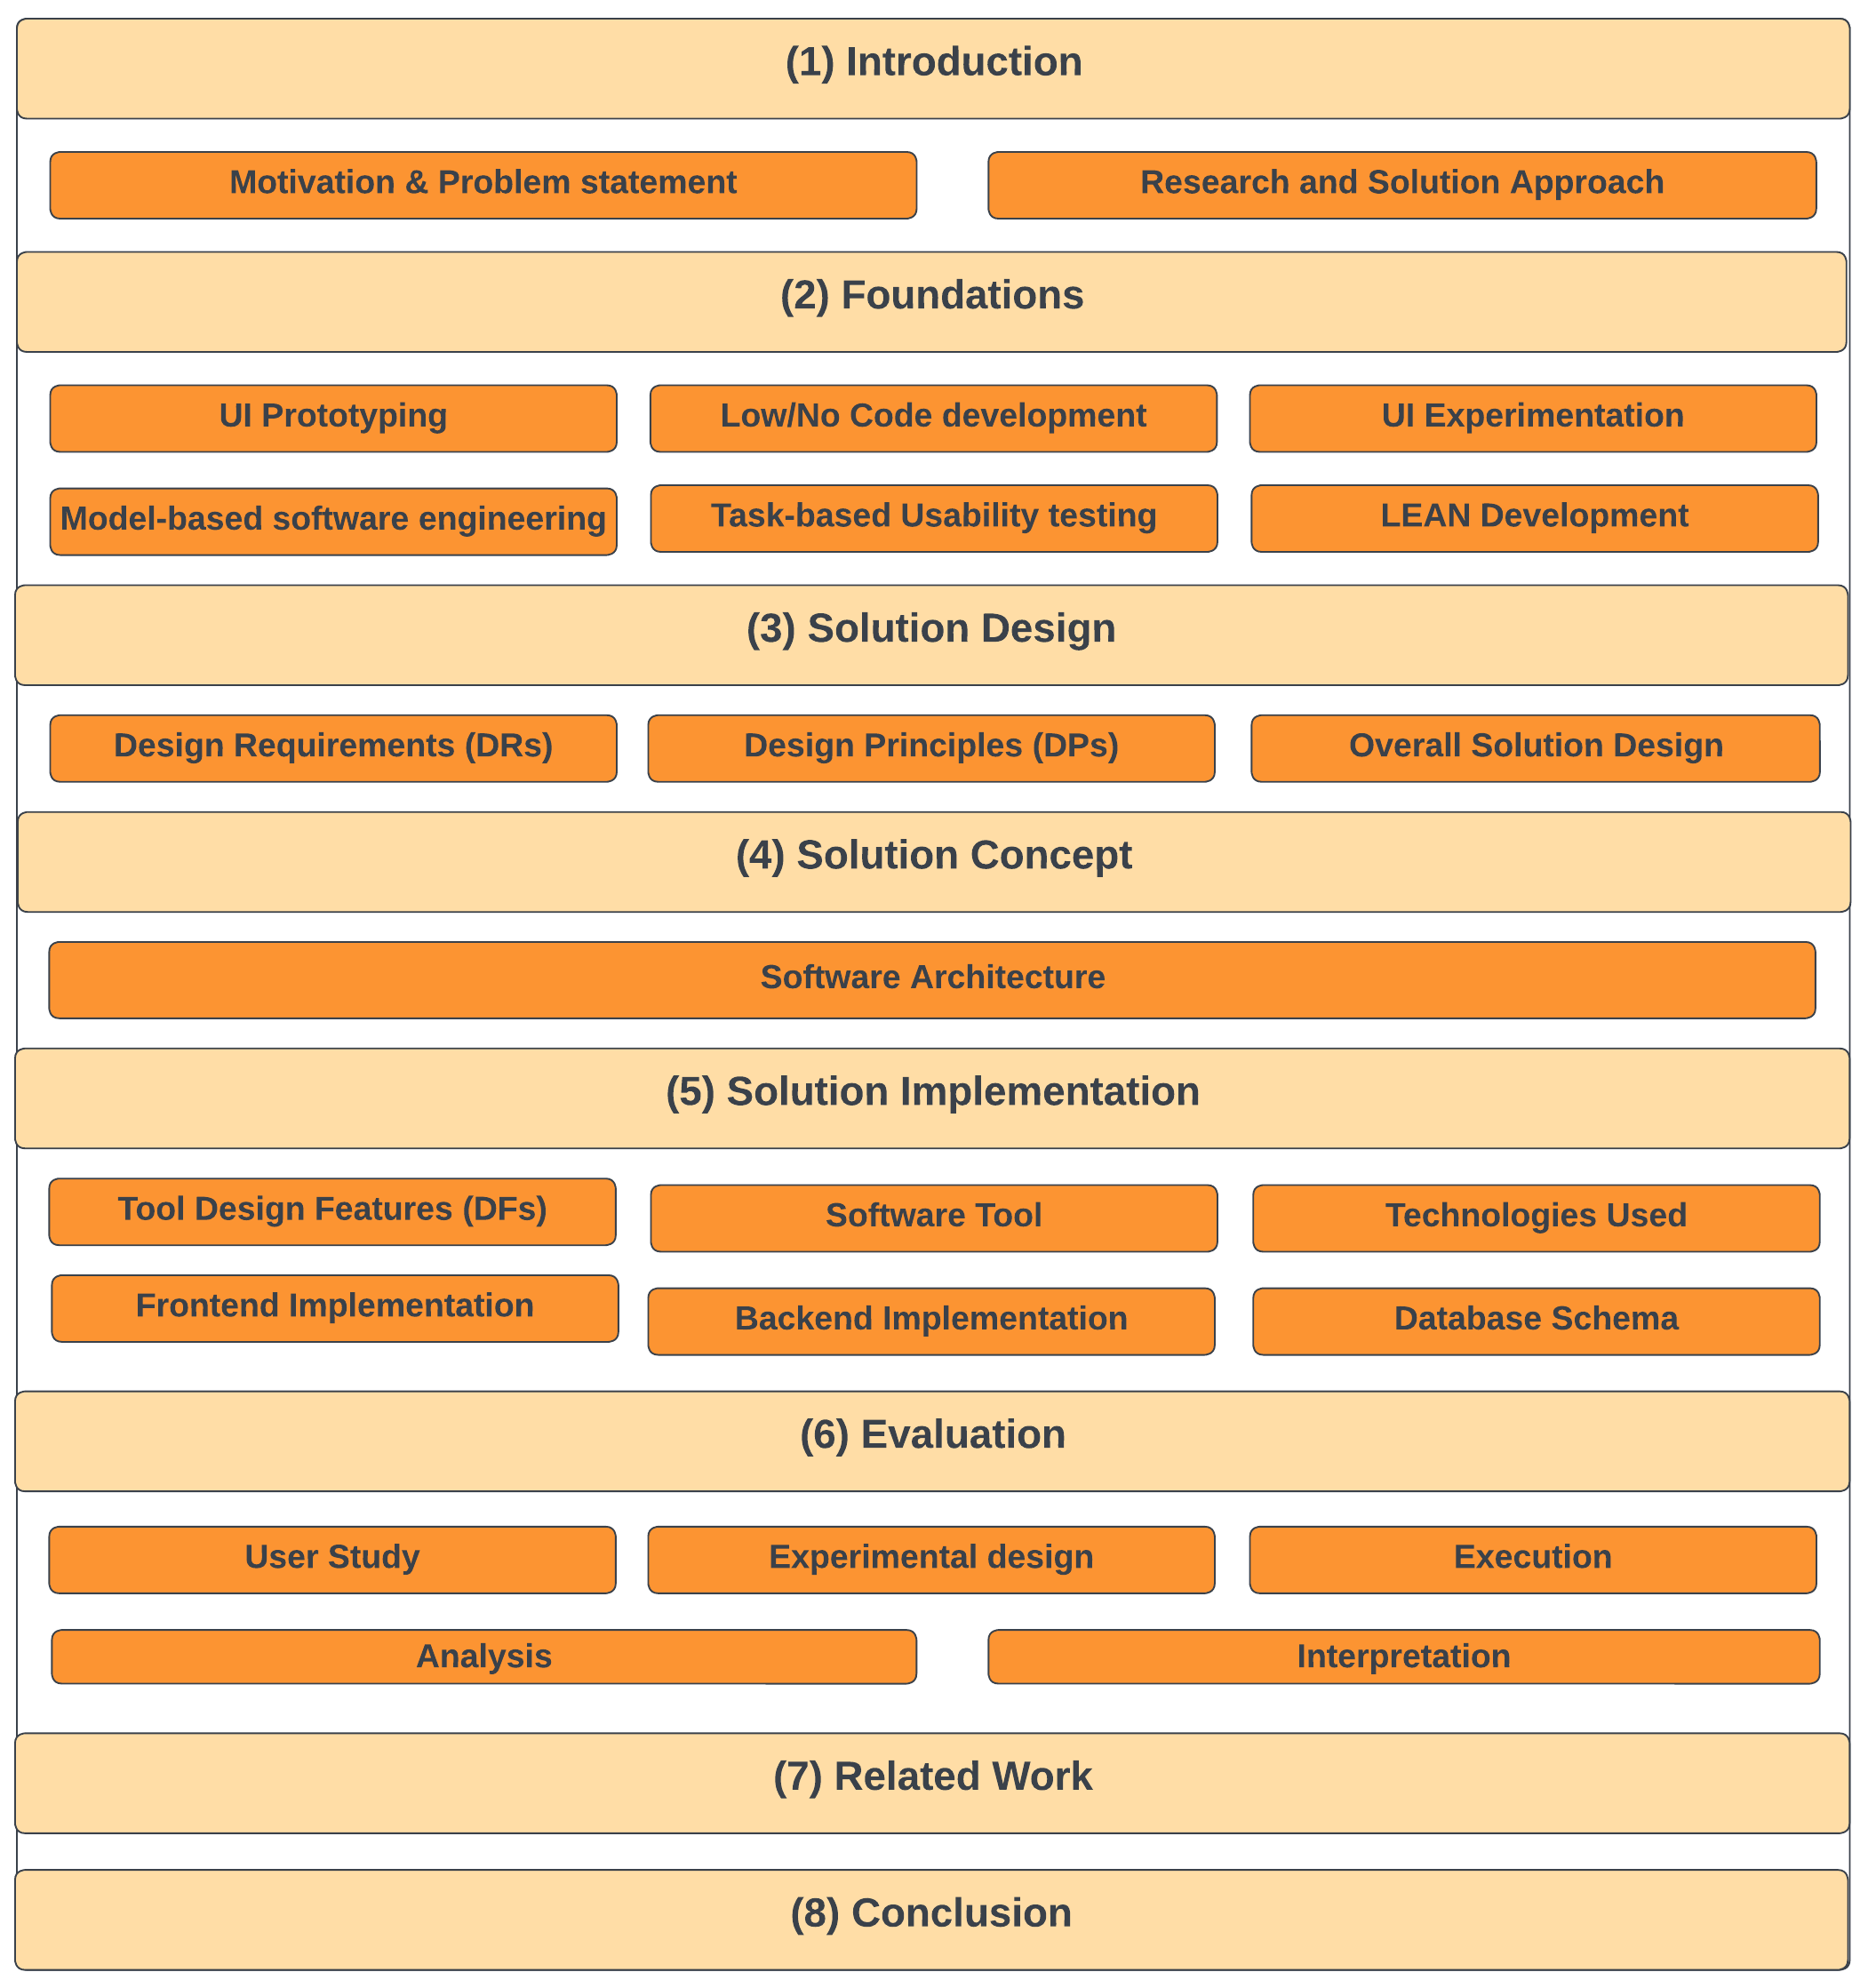
\includegraphics[scale=0.2]{Structure.png}
    \caption{Thesis Structure}
    \label{intro:fig:structure}
\end{figure}

Next, the \textit{\hyperref[chap:foundations]{(2) Foundations}} chapter is used to gain the knowledge required to understand the scope of our work, which includes \ac{ui} prototyping, low/no-code development, model-based software engineering, task-based usability testing, \ac{ui} experimentation, and LEAN development.
The \textit{\hyperref[chap:design]{(3) Solution Design}} chapter outlines the \ac{dr}s, \ac{dp}s, and overall solution design. 
Similarly, the \textit{\hyperref[chap:concept]{(4) Solution Concept}} chapter presents the software architecture, \ac{ui} prototype management, \ac{ui} experimentation management, persistence components, deployment components, and security components.
Next, the \textit{\hyperref[chap:implementation]{(5) Solution Implementation}} chapter provides detailed insights into the tool \ac{df}s, explains the software tool we developed, technologies used, frontend and backend implementation, and database schema. 
Next, the \textit{\hyperref[chap:evaluation]{(6) Evaluation}} chapter showcases the user study, experimental design, execution, analysis, and interpretation. 
Next, the \textit{\hyperref[chap:relatedWork]{(7) Related Work}} section discusses current tools and state-of-the-art technologies and compares them with our \ac{dr}s.
Finally, in the \textit{\hyperref[chap:conclusion]{(8) Conclusion}} chapter, we summarize our work, future work, and research contributions.
